\chapter{Bilans}

\section{Planning effectif du projet}

\begin{figure}[h]
    \centering
    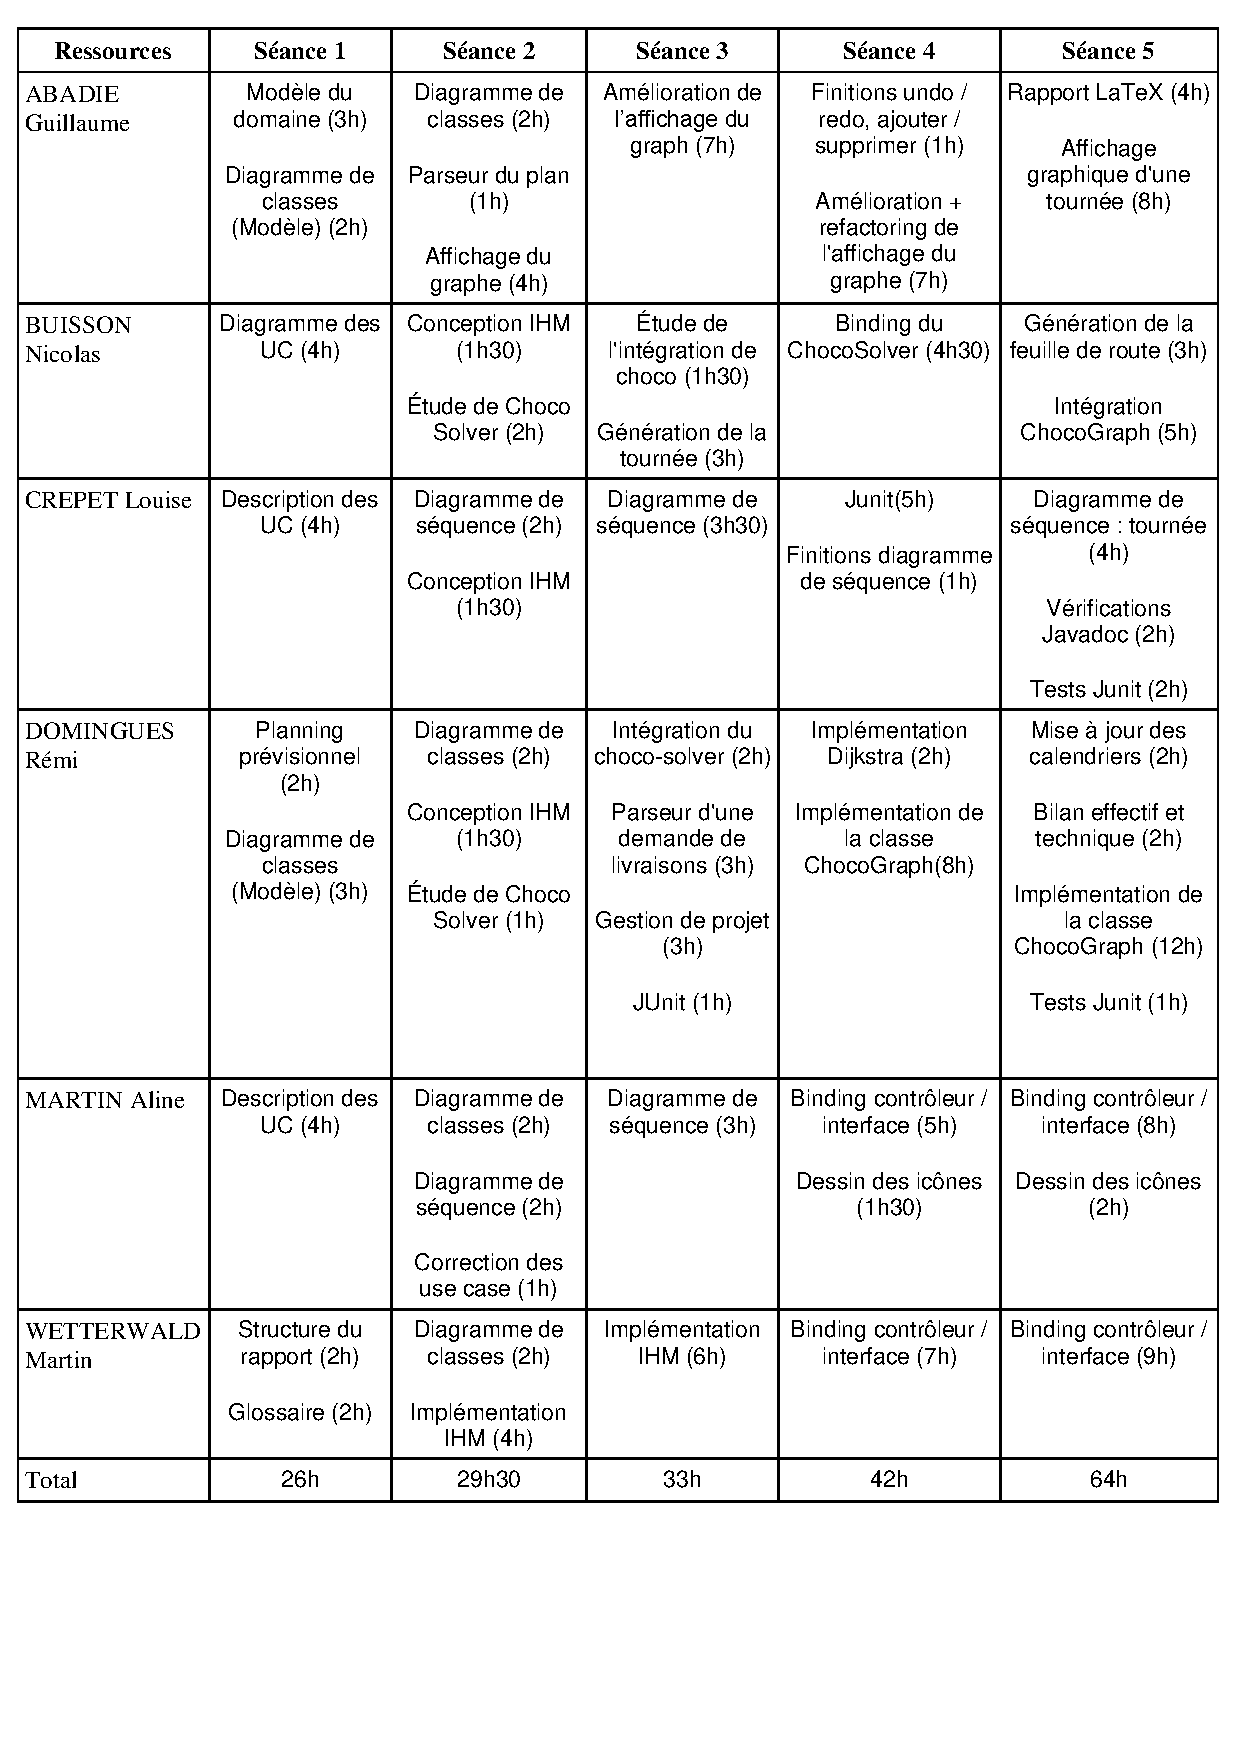
\includegraphics[width=130mm]{../diagrams/project_management/planning_effectif/planning_horaire.pdf}
    \caption{Planning horaire du projet}
    \label{diagram:planning_horaire}
\end{figure}
\pagebreak

\begin{landscape}
\begin{figure}[h]
    \centering
    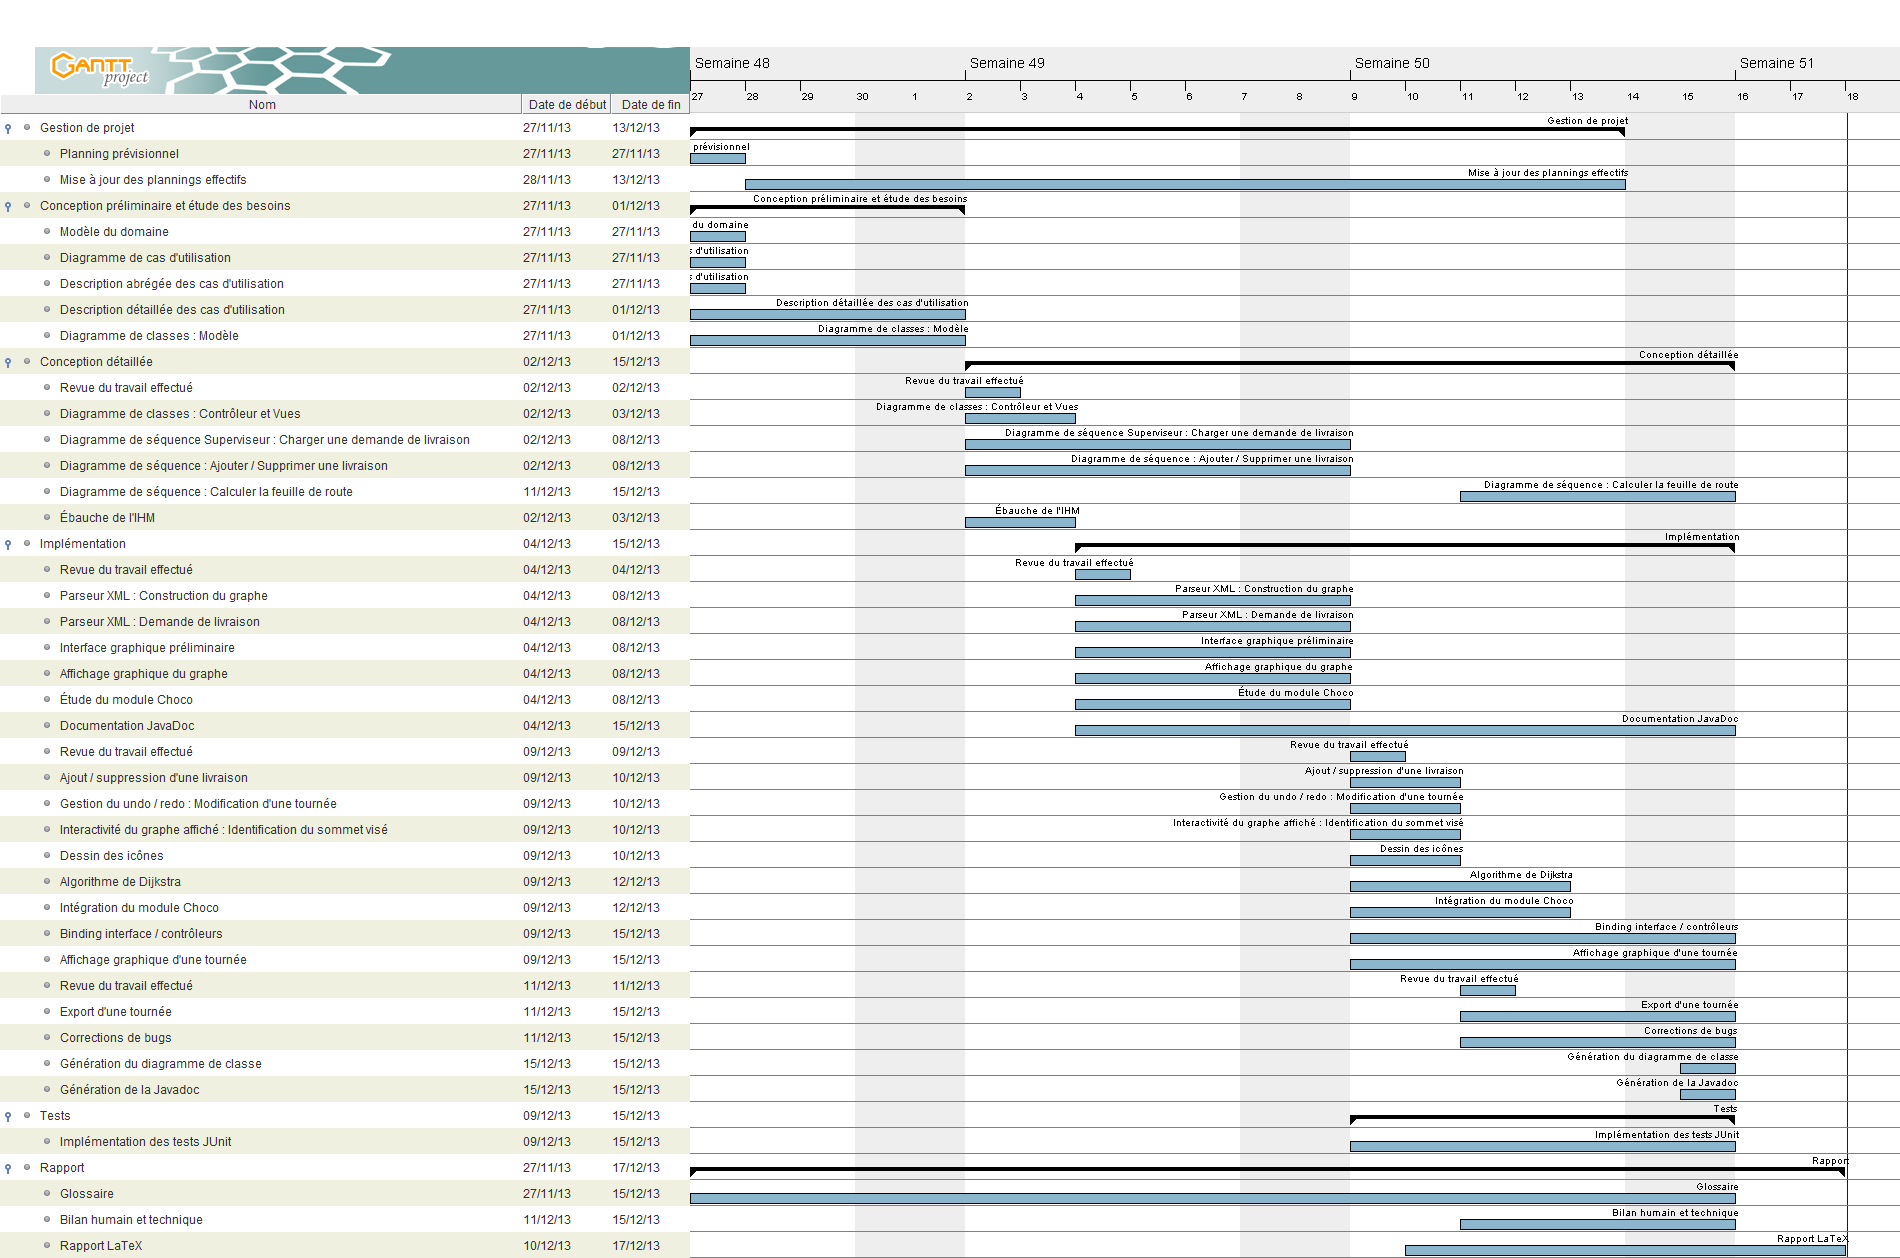
\includegraphics[width=240mm]{../diagrams/project_management/planning_effectif/planning_effectif.png}
    \caption{Planning effectif du projet}
    \label{diagram:planning_effectif}
\end{figure}
\end{landscape}
\pagebreak

\begin{landscape}
\begin{figure}[h]
    \centering
    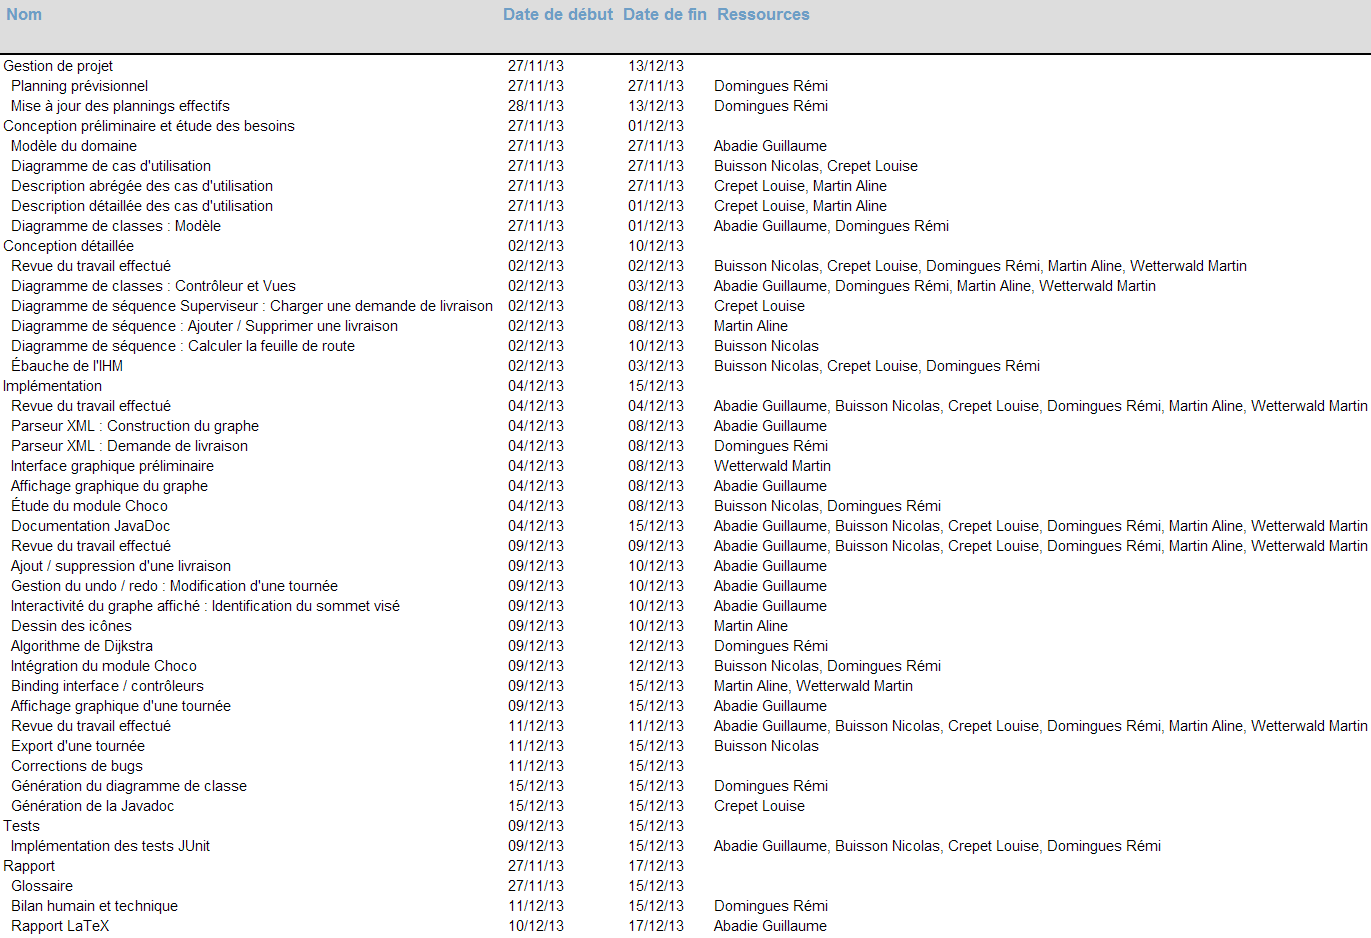
\includegraphics[width=220mm]{../diagrams/project_management/planning_effectif/tasks_repartition.png}
    \caption{R\'epartition des t\^aches}
    \label{diagram:tasks_repartition}
\end{figure}
\end{landscape}
\pagebreak

\begin{landscape}
\begin{figure}[h]
    \centering
    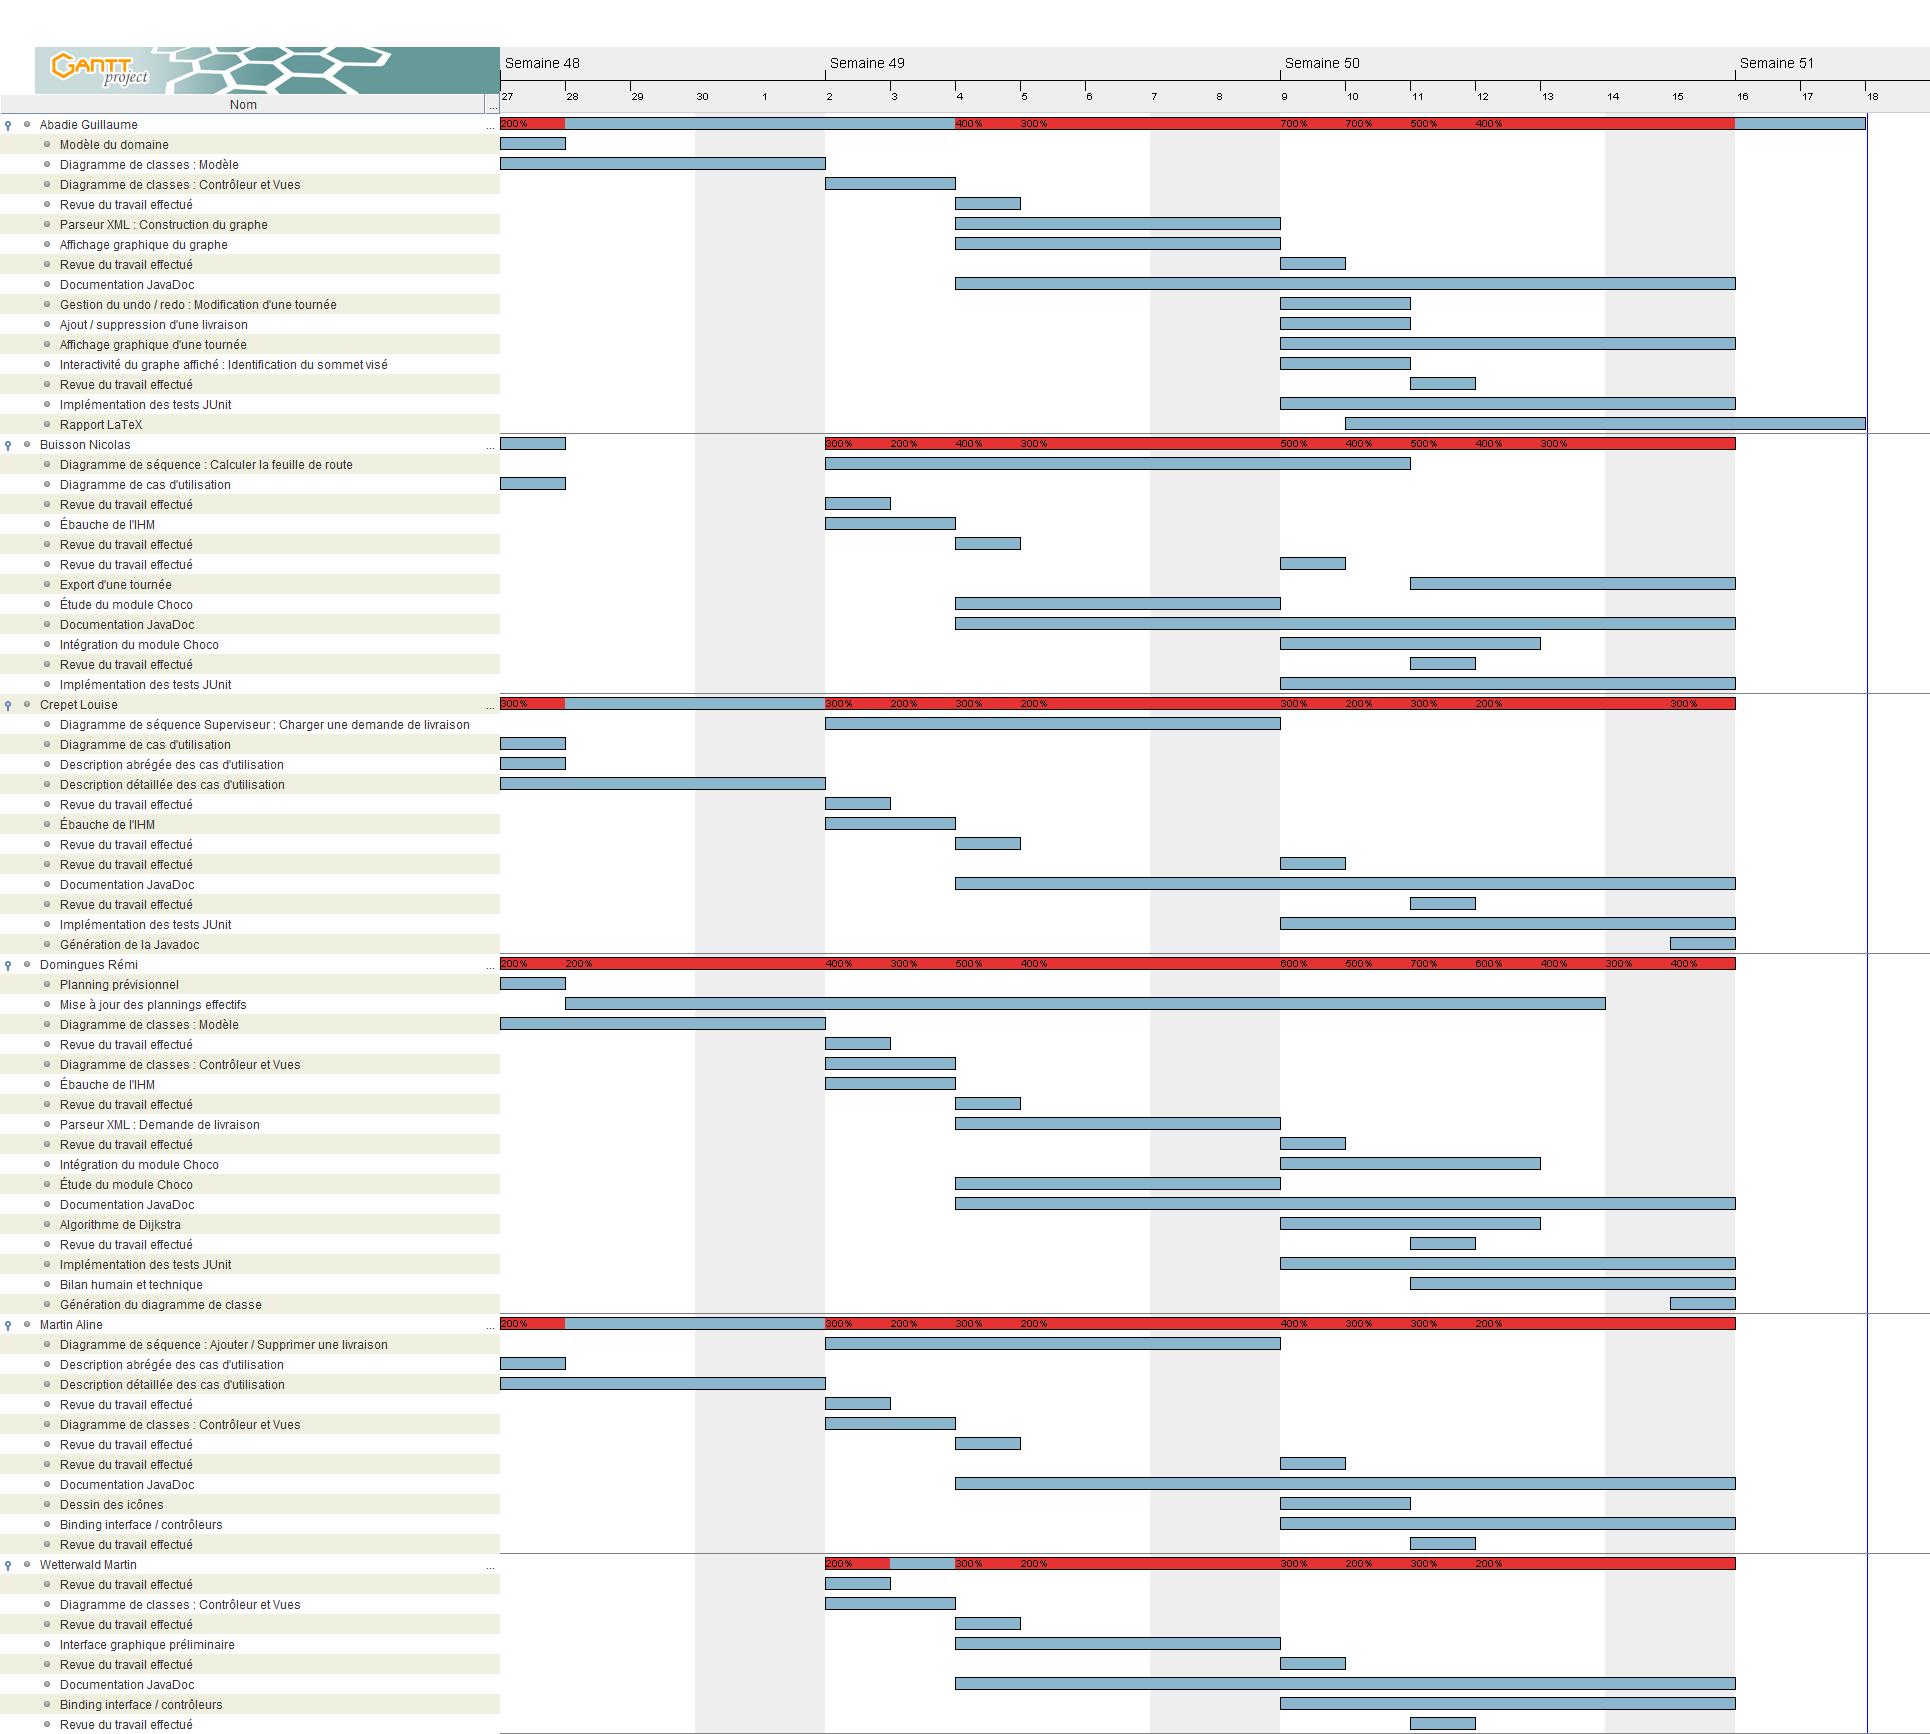
\includegraphics[width=180mm]{../diagrams/project_management/planning_effectif/planning_ressources.png}
    \caption{Planning des ressources du projet}
    \label{diagram:planning_ressource}
\end{figure}
\end{landscape}
\pagebreak


\section{Bilan humain}
\subsection{Méthodologie}
La réalisation du projet Opti\_fret\_COURLY est une occasion idéale pour l’exercice des méthodologies enseignées dans la filière Informatique de l’INSA de Lyon. Celle-ci permit en effet une importante gestion de projet (diagramme de Gantt et de ressources, évaluation des durées des tâches, répartition des rôles, gestion du planning afin de respecter les échéances critiques) et une collaboration entre les différents membres de l’équipe de projet. Ce fut également l’occasion de réaliser un système en collaboration avec un client tenant rôle de maître d’ouvrage, permettant à notre équipe de se rendre compte de l’importance du dialogue avec le client, mais également de la position centrale que doivent occuper ses besoins dans la conception et la réalisation d’une application.

\subsection{Respect du planning et adaptations}
L’efficacité d’une équipe dynamique, sérieuse et bien organisée permit un respect certain des échéances fixées et du planning général. Si, comme escompté, de nombreuses tâches ne purent être effectuées dans le cadre d’une séance de travail, celles-ci furent systématiquement ou presque terminées en dehors des heures pédagogiques.

\subsection{Ressenti}
La première difficulté rencontrée dans la réalisation de ce projet est celle de la continuité du projet IHM. Le projet DevOO semble en effet présenté comme la réalisation du projet précédent, basé sur le même sujet récapitulatif des besoins clients. L'appréhension de nouveaux besoins clients est alors nécessaire.

Il est en outre demandé de réaliser une conception d'application en désaccord avec sa réalisation (diagrammes de cas d'utilisation incluant les applications livreurs et une base de données), ajoutant au sentiment de désarroi de l'équipe de projet.

Enfin, les fichiers XML de description d'un plan et d'une livraison étant livrés sans schéma XML ou DTD associée, la réalisation des parseurs en est approximative et l'exercice de réalisation d'un tel parseur en accord avec une DTD n'est pas pratiqué.
\clearpage

\section{Bilan technique}
\subsection{Sujet}
La réalisation de ce système tire son intérêt majeur du projet réel dont il est issu. Il s’agit en effet là d’une application utilitariste basée sur un cas d’utilisation concret en accord avec les projets futurs que chacun d’entre nous devra réaliser dans un cadre professionnel.

En outre, ce sujet aborde des domaines techniques d'intérêt tels l'affichage graphique d'un graphe interactif, la résolution d'un plus court chemin dans un graphe et la résolution d'un TSP (traveler salesman problem).

\subsection{Compétences acquises}
Ce projet de est en premier lieu l'occasion pour un hexanôme d'approfondir ses compétences en développement dans un langage de programmation de son choix.

Par ailleurs, celui-ci permet la découverte ou l'approfondissement de l'utilisation de bibliothèques graphiques standards dans le cadre du dessin d'un graphe, s'accompagnant de calculs vectoriels et de gestion des événements de la fenêtre parente.

Il en est enfin de même vis-à-vis de l'algorithme de Dijkstra permettant de calculer des plus courts chemins, et de la librairie interfaçant Choco fournie permettant la résolution d'un TSP. L'acquisition et la connaissance du maniement d'une telle librairie sera sans nul doute d'une indéniable utilité dans le cadre de la carrière future de certains membres de notre hexanôme.
\clearpage
